% !TEX root = SystemTemplate.tex
\chapter{User Stories, Backlog and Requirements}
\section{Overview}

This section covers user stories, backlog and requirements for the system.  

\subsection{Scope}

This document contains stakeholder information, 
initial user stories, requirements, proof of concept results, and various research 
task results. 



\subsection{Purpose of the System}
The purpose of the product is to grade a {\tt <filename>.cpp} file by running test files and comparing the results to answer files, and assigning percentage grade. 


\section{ Stakeholder Information}


This section would provide the basic description of all of the stakeholders for 
the project.

\subsection{Customer or End User (Product Owner)}
Hafiza Farzami is the product owner for this sprint, who is in contact with Dr. Logar regarding requirements, and with the scrum master and technical lead regarding the backlog. 

\subsection{Management or Instructor (Scrum Master)}
Julian Brackins is the scrum master, who breaks the project into smaller tasks, and is in touch with both product owner and technical lead.

%\subsection{Investors}
%Are there any?  Who?  What role will they play? 

\subsection{Developers --Testers}
Jon Dixon is the technical lead for Sprint 2, and is in contact with both Brackins and Farzami regarding the requirements during scrum meetings and through trello notes. Due to the project size and limited number of people, the developers and testers are the same group of people. 

\section{Business Need}
This product is essential for grading computer science programs focused on numerics. The user can save time and not have to do tedious, meticulous work while grading an entire class of students' programs.  

\section{Requirements and Design Constraints}
This section covers the requirements and constraints in order to use this product. 

\subsection{System  Requirements}
This product runs on Linux machines. 

\subsection{Network Requirements}
This software does not require internet connection. 

\subsection{Development Environment Requirements}
There are not any development environment requirements.

\subsection{Project  Management Methodology}
The method used to manage this project is {\tt scrum}. The scrum master met with the product owner, and broke the tasks down to the technical lead. The team meets for ten minutes long scrum meetings to go over the progress, next steps, and impediments. 
 
\begin{itemize}
\item Trello is used to keep track of the backlogs and sprint status
\item Everyone has access to the Sprint and Product Backlogs
\item This project will take three Sprints
\item Each Sprint is two weeks long
\item There are no restrictions on source control 
\end{itemize}

\section{User Stories}
This section contains the user stories regarding functional requirements and how the team broke them down.

\subsection{User Story}
As user I want a testing system, in C++,  so that given a directory of a class containing {\tt <studentsNames>.cpp} files and a test files, it should grade them. 

\subsubsection{User Story Breakdown \#1}
The program needs to be able to "crawl" through directories, be able to identify and run {\tt <studentsNames>.cpp} files using the test files. In other words, the testing suite should be able to process the entire class. 

\begin{figure}[tbh]
\begin{center}
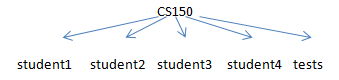
\includegraphics[width=0.75\textwidth]{./Capture}
\end{center}
\caption{Directory Hiararchy Structure \label{directoryhiararchystructure}}
\end{figure}

\subsubsection{User Story Breakdown \#2}
The system needs to grade each individual student, store the result in a log file specific to a given student. The system also has to produce a summary file containing the list of grade percentages of all the students who passed necessary test cases, and the students who failed to pass an important critical case, with the word "FAILED" in the grade column.

\subsubsection{User Story Breakdown \#3}
The individual {\tt <studentName>.log} files will be stored in that student's subdirectory. The summary {\tt .log} file will be located in the root directory.  

The summary file will have the following structure: \\*
\newline
\indent	Student1 Name	\indent Percent grade {\tt or} FAILED \\*
\indent	Student2 Name	\indent Percent grade {\tt or} FAILED \\*
\indent \indent \indent \indent \indent \indent	.				 \\*
\indent \indent \indent \indent \indent \indent	.				 \\*
\indent \indent \indent \indent \indent \indent	.				 \\*
\indent	Studentn Name	\indent Percent grade {\tt or} FAILED
	

\subsubsection{User Story Breakdown \#4}
The system should be able to generate test cases by asking the user about the conditions and constraints.

\let\cleardoublepage\clearpage

